\documentclass[a4paper, 10pt, fleqn]{article}

\usepackage{layout}

\title{TKOM - Signale und Systeme}
\author{daniw}
\date{\today}

\begin{document}

\maketitle

\clearpage

\tableofcontents

\clearpage

\section{SW01}
\subsection{Anwendung}
\begin{itemize}
    \item Speicherung von Informationen
    \item Informationsübertragung
    \item Extraktion von Information
    \item Detektion von Ereignissen
\end{itemize}
\subsection{Buch}
Signal- und Systemtheorie - Thomas Frey, Martin Bossert \\
Online verfügbar in HSLU Bibliothek

\section{Einleitung}
\begin{tabular}{|l|l|l|l|}
\hline                         &                   & \multicolumn{2}{|c|}{Amplitude} \\
\hline                         &                   & kontinuierlich    & diskret \\
\hline \multirow{2}{*}{Zeit}   & kontinuierlich    & analog            & \\
\cline{2-4}                    & diskret           &                   & digital   \\
\hline
\end{tabular}

Kontinuierliches System: 
\[ y(t) = H\{x(t)\} \]
Diskretes System: 
\[ y[k] = H\{x[k]\} \qquad k \in \mathbb{N} \]

\subsection{Systeme}
Lineares System: 
\[ H\{a_1 x_1(t) + a_2 x_2(t)\} = a_1 H\{x_1(t)\} + a_2 H\{x_2(t)\}, \qquad a_1, a_2 \in \mathbb{R}(\mathbb{C}) \]
Zeitinvariantes System: 
\[ y(t - t_0) = H\{x(t - t_0)\} \]
LTI-System: linear und zeitinvariant \\\\
Kausales System: 
\[ y(t_0) = H\{x(t \leq t_0)\} \]
Stabilas System:
\[ |x(t)| < \infty \Rightarrow |H\{x(t)\}| < \infty \]

\subsubsection{Beispiele}
Signal $x(t)$ \\
$x(t - \tau$ ist die umf $\tau$ verzögerte Version von $x(t)$. \\\\
\[
    y(t) = \left\{
    \begin{array}{lll}
        x(t) & \text{für} 0 \leq t \leq 1 \\
        0    & \text{für} t < 0, t = 1 \\
    \end{array}
    \right.
\]
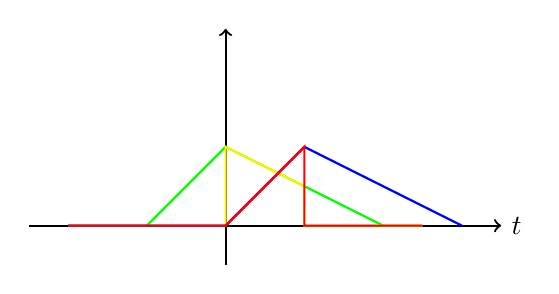
\begin{tikzpicture}
    \draw[thick, ->]        (-2.5,0) -- (3.5,0) node[right] {$t$};
    \draw[thick, ->]        (0,-0.5) -- (0,2.5);
    \draw[thick, green]     (-2,0) -- (-1,0) -- (0,1) -- (2,0) -- (2.5,0);
    \draw[thick, yellow]    (-2,0) -- (0,0) -- (0,1) -- (1,0.5) -- (1,0) -- (2.5,0);
    \draw[thick, blue]      (-2,0) -- (0,0) -- (1,1) -- (3,0);
    \draw[thick, red]       (-2,0) -- (0,0) -- (1,1) -- (1,0) -- (2.5,0);
\end{tikzpicture}\\
$\to$ nicht zeitinvariant $\to$ kein LTI-System

\section{Signale}
Zeitliche Verschiebung
\[ x(t - t_0) \]
Zeitliche Spiegelung
\[ x(-t) \]
Zeitliche Skalierung
\[ x(a \cdot t) \]
Komplexe Signale
\[ x(t) = x_R(t) + j \cdot x_I(t) = Re(x(t)) + j \cdot Im(x(t)) = |x(t)| \cdot e^{j \angle x(t)} \]
Gerade Signale
\[ x(t) = x(-t) \]
Ungerade Signale
\[ x(t) = -x(-t) \]
Zerlegung in geraden und ungeraden Anteil
\[ x_g(t) = \frac{1}{2} \cdot \left(x(t) - x(-t)\right) \]
\[ x_u(t) = \frac{1}{2} \cdot \left(x(t) + x(-t)\right) \]
\[ x(t) = x_g(t) + x_u(t) \]
Konjugiert gerade Signale
\[ x(t) = x^{\star}(-t) \]
Konjugiert ungerade Signale
\[ x(t) = -x^{\star}(-t) \]
Periodische Signale
\[ x(t) = x(t + n \cdot T_p) \qquad n \in \mathbb{Z} \]
Zeitbegrenzte Signale
\[ x(t) = 0 \qquad \text{für $t < t_1$ oder $t > t_2$} \]

\subsection{Spezielle Signale}
Zeitdiskreter Dirac-Impuls
\[
\sigma[k] = \left\{
    \begin{array}{ll}
        1, & k = 0 \\
        0, & k \neq 0
    \end{array}
\right.
\]
Zeitdiskrete Sprungfunktion
\[
\varepsilon[k] = \left\{
    \begin{array}{ll}
        1, & k \geq 0 \\
        0, & k < 0
    \end{array}
\right.
\]
Kontinuierliche Sprungfunktion
\[
\varepsilon(t) = \left\{
    \begin{array}{ll}
        1, & t > 0 \\
        0, & t < 0
    \end{array}
\right.
\]
Zeitdiskrete Signumfolge
\[
\sgn[k] = \left\{
    \begin{array}{ll}
        1,  & k > 0 \\
        0,  & k = 0 \\
        -1, & k < 0
    \end{array}
\right.
\]
Kontinuierlicher Rechteckimpuls
\[
\rect_T(t) = \left\{
    \begin{array}{ll}
        1, & |t| < \frac{T}{2} \\
        0, & |t| > \frac{T}{2}
    \end{array}
\right.
\]
Reelle Exponentialfunktion
\[ x(t) = A \cdot e^{\alpha t} \qquad \alpha < 0 \to \text{ abklingend} \qquad \alpha > 0 \to \text{ aufklingend} \]
Komplexe Exponentialfunktion
\[ x(t) = A \cdot e^{\alpha t} \cdot e^{j \omega_0 t} = \underbrace{|A| \cdot e^{\sigma t}}_{\text{Einhüllende}} \cdot \underbrace{e^{j(\omega_0 t + \varphi_0)}}_{\text{komplexe Schwingung}} \]
si-Funktion
\[ \si(t) = \frac{\sin(t)}{t} \]

\section{Energie, Leistung}
Energie
\[ E_x = \sum\limits_{k = -\infty}^{\infty} \left(\left|x[k]\right|^2\right) \]
\[ E_x = \int\limits_{-\infty}^{\infty} \left(\left|x(t)\right|^2\right) dt \]
Energiesignale: 
\[ E_x < \infty \]
Leistung
\[ P_x = \lim\limits_{n \to \infty} \frac{1}{2 \cdot n + 1} \sum\limits_{k = -n}^{n} \left(\left|x[k]\right|^2\right) \]
\[ P_x = \lim\limits_{T \to \infty} \frac{1}{T} \int\limits_{-\frac{T}{2}}^{\frac{T}{2}} \left(\left|x(t)\right|^2\right) dt \]
Leistungssignale:
\[ P_x > 0 \qquad P_x < \infty \]

\section{Korrelation von Energiesignalen}

\subsection{Kreuzkorrelation}
\[ \varphi_{xy}^{E} (\kappa) = \sum\limits_{k = -\infty}^{\infty} \left(x^\star[k] \cdot y[k + \kappa]\right) \]
\[ \varphi_{xy}^{E} (\tau) = \int\limits_{-\infty}^{\infty} \left(x^\star(t) \cdot y(t + \tau)\right) dt \]
es gilt: 
\[ \varphi_{yx}(\tau) = \varphi_{xy}^\star(-\tau) \]

\subsection{Autokorrelation}
\[ \varphi_{xx}^{E} (\kappa) = \sum\limits_{k = -\infty}^{\infty} \left(x^\star[k] \cdot x[k + \kappa]\right) \]
\[ \varphi_{xx}^{E} (\tau) = \int\limits_{-\infty}^{\infty} \left(x^\star(t) \cdot x(t + \tau)\right) dt \]
es gilt: 
\[ E_x = \varphi_{xx}^{E} (0) \]

\section{Korrelation von Leistungssignalen}

\subsection{Kreuzkorrelation}
\[ \varphi_{xy}^{L} (\kappa) = \lim\limits_{n \to \infty} \frac{1}{2 \cdot n + 1} \sum\limits_{k = -n}^{n} \left(x^\star[k] \cdot y[k + \kappa]\right) \]
\[ \varphi_{xy}^{L} (\tau) = \lim\limits_{T \to \infty} \frac{1}{2 \cdot T} \int\limits_{-T}^{T} \left(x^\star(t) \cdot y(t + \tau)\right) dt \]
es gilt: 
\[ P_x = \varphi_{xx}^{L} (0) \]

\subsection{Kreuzkorrelation periodischer Signale}
\[ \varphi_{xy}^{L} (\kappa) = \frac{1}{N_p} \sum\limits_{k = k_0}^{k_0 + N_p - 1} \left(x^\star[k] \cdot y[k + \kappa]\right) \]
\[ \varphi_{xy}^{L} (\tau) = \frac{1}{T_p} \int\limits_{t_0}^{t_0 + T_p} \left(x^\star(t) \cdot y(t + \tau)\right) dt \]

\section{Geometrische Reihe}
\[ \sum\limits_{k = 0}^{\infty} q^k = \frac{1}{1 - q} \]

\section{Diskrete LTI Systeme}
\[ y[k] = y[k - 1] + y[k - 2] + x[k] \qquad x[k] = \delta[k] \]

\subsection{Differenzengleichung in allgemeiner Form}
\[ y[k] = -\sum\limits_{i = 1}^{n} \~{a_i} ~ y[k - i] + \sum\limits_{i = 1}^{\ell} \tilde{b_i} ~ y[k - \ell] \]

\subsubsection*{Beispiel Hasenzucht}
\[ y[k] = y[k - 1] + y[k - 2] + x[k] \qquad x[k] = \delta[k] \]
\[ 
    \underbrace{\sum\limits_{k = -\infty}^{\infty} y[k] \cdot z^{k}}
    _{Y(z)}
    =
    \underbrace{\sum\limits_{k = -\infty}^{\infty} y[k - 1] \cdot z^{k}}
    _{z^{-1} \cdot \sum\limits_{k = -\infty}^{\infty} y[k - 1] \cdot z^{-(k - 1)} = z^{-1} \cdot Y(z)}
    +
    \underbrace{\sum\limits_{k = -\infty}^{\infty} y[k - 2] \cdot z^{k}}
    _{z^{-2} \cdot Y(z)}
    +
    \underbrace{\sum\limits_{k = -\infty}^{\infty} x[k] \cdot z^{k}}
    _{X(z)}
\]
\[ Y(z) = z^{-1} \cdot Y(z) + z^{-2} \cdot Y(z) + X(z) \]
\[ Y(z) = \frac{1}{1 - z^{-1} - z^{-2}} \cdot X(z) \]
\[ x[k] = \delta[k] ~\laplace~ X(z) = \sum\limits_{k = -\infty}^{\infty} x[k] \cdot z^{-k} = 1 \]
\[ \rightarrow Y(z) = \frac{1}{1 - z^{-1} - z^{-2}} \]
\[ \rightarrow Y(z) = \frac{z^2}{z^2 - z - 1} = z \cdot \frac{z}{z^2 - z - 1} \]
Partialbruchzerlegung von $\frac{z}{z^2 - z - 1}$
\[ \frac{z}{z^2 - z - 1} = \frac{A}{z - a} + \frac{B}{z - b}
= \frac{A \cdot (z - b) + B \cdot (z - a)}{(z - a) \cdot (z - b)}\]
\[ z^2 - z - 1 = (z - a) \cdot (z - b) \]
\[ z^2 - z - 1 = 0 \qquad \text{für } z_{1,2} = \frac{1}{2} \pm \sqrt{\frac{1}{4} + 1}
    \to \left\{ 
    \begin{array}{l} 
        a = \frac{1}{2} \left(1 + \sqrt{5}\right) \\
        b = \frac{1}{2} \left(1 - \sqrt{5}\right) 
    \end{array} \right.
\]
\[ z = A \cdot (z - b) + B \cdot (z - a) \]
\[ z = A \cdot z + B \cdot z - A \cdot b - B \cdot a \]
\[ \left. \begin{array}{l}
        A + B = 1 \\
        A \cdot b + B \cdot a = 0
    \end{array} \right\} 
    \to \boxed{A = \frac{1}{2} \cdot \left(1 + \frac{1}{\sqrt{5}}\right),
    B = \frac{1}{2} \cdot \left(1 - \frac{1}{\sqrt{5}}\right) }
\]
Einsetzen
\[ Y(z) = \frac{A \cdot z}{z - a} + \frac{B \cdot z}{z - b} 
= \frac{A}{1 - \frac{a}{z}} + \frac{B}{1 - \frac{b}{z}}\]
\[ \sum\limits_{k = 0}^{\infty} q^k = \frac{1}{1 - q} \qquad \forall ~ |q| < 1 \]
\[ \to \frac{1}{1 - \frac{a}{z}} = \sum\limits_{k = 0}^{\infty} \left(\frac{a}{z}\right)^k
= \sum\limits_{k = 0}^{\infty} a^k \cdot z^{-k} \]
\[ Y(z) = A \cdot \sum\limits_{k = 0}^{\infty} a^k \cdot z^{-k} + B \cdot \sum\limits_{k = 0}^{\infty} b^k \cdot z^{-k} \]
\[ y[k] = \left( A \cdot a^k + B \cdot b^k \right) \cdot \varepsilon[k] \]

\subsection{z-Transformation}
Definition:
\[ X(z) = Z\{x[k]\} = \sum\limits_{k = -\infty}^{\infty} x[k] \cdot z^{-k} \qquad z \in \mathbb{C} \]
Korrespondenzen: 
\[ Z\{\delta[k]\} = 1 \qquad \text{Impulsfolge} \]
\[ Z\{a^k \cdot \varepsilon[k]\} = \frac{z}{z - a} \qquad \text{kausale Exponentialfolge} \]
Verschiebungsregel:
\[ Z\{x[k - k_0]\} = z^{-k_0} \cdot Z\{x[k]\} \]
Schreibweise:
\[ x[k] \laplace X(z) \]

\subsubsection{Herleitung einer geschlossenen Lösung über die z-Transformation}
Differenzengleichung: 
\[ y[k] = y[k - 1] + y[k - 2] + x[k] \]
Transformation in z-Bereich:
\[ Y(z) = \frac{X(z)}{1 - z^{-1} - z^{-2}} = \frac{z^2}{z^2 - z^1 - z} \]
Partialbruchzerlegung: 
\[ Y(z) = \frac{A \cdot z}{z - a} + \frac{B \cdot z}{z - b} \]
Rücktransformation in Zeitbereich:
\[ y[k] = \left[ A \cdot a^k + B \cdot b^k \right] \cdot \varepsilon[k] \]

\subsubsection{Beschreibung allgemeiner LTI-Systeme im z-Bereich}
Differenzengleichung:
\[ y[k] = -\sum\limits_{i = 1}^{n} \tilde{a}_i \cdot y[k - i] + \sum\limits_{\ell = 1}^{m} \tilde{a}_i \cdot y[k - \ell] \]
elementweise Transformation:
\[ \begin{array}{ccc}
    \sum\limits_{i = 0}^{n} \tilde{a}_i \cdot y[k - i] & 
        = & 
        \sum\limits_{i = 1}^{m} \tilde{b}_i \cdot y[k - i] \\
    \laplace &   & \laplace \\
    \sum\limits_{i = 0}^{n} \tilde{a}_i \cdot z^{-i} \cdot Y(z) & 
        = & 
        \sum\limits_{i = 1}^{m} \tilde{b}_i \cdot z^{-i} \cdot Y(z) \\
\end{array} \]
Ausgabesignal im z-Bereich:
\[ Y(z) = \frac{\sum\limits_{i = 0}^{m} \tilde{b}_i \cdot z^{-i}}
    {\sum\limits_{i = 0}^{m} \tilde{a}_i \cdot z^{-i}} 
    \cdot X(z) = H(z) \cdot X(z) \qquad \tilde{a} \neq 0
\]

\subsection{Übertragungsfunktion und Impulsantwort}
Übertragungsfunktion (Systemantwort):
\[ H(z) = \frac{Y(z)}{X(z)} 
    = \frac{\sum\limits_{i = 0}^{m} \tilde{b}_i \cdot z^{-i}}
    {\sum\limits_{i = 0}^{n} \tilde{a}_i \cdot z^{-i}}
    = \frac{\tilde{b}_0 + \tilde{b}_1 \cdot z^{-1} + \ldots + \tilde{b}_m \cdot z^{-m}}
    {\tilde{a}_0 + \tilde{a}_1 \cdot z^{-1} + \ldots + \tilde{a}_n \cdot z^{-n}}
    \qquad \tilde{a}_0 \neq 0 \]
Impulsantwort:
\[ h[k] = H\{ \delta[k] \} ~ \laplace ~ H(z) \]

\subsection{Beispiel Funkstrecke}
\[ y[k] = x[k] + \frac{1}{2} \cdot x[k - 1] \]
\[ Y(z) = X(z) + \frac{1}{2} \cdot z^{-1} \cdot X(z) \]
\[ Y(z) = \left( 1 + \frac{1}{2} \cdot z^{-1} \right) \cdot X(z) \]
\[ H(z) = 1 + \frac{1}{2} \cdot z^{-1} \]
\[ h[k] = \delta[k] + \frac{1}{2} \cdot \delta[k - 1] \]

\subsection{Beispiel Hasenzucht mit Koeffizienten}
\[ y[k] = y[k-1] + y[k-2] + x[k] \]
\[ H(z) = \frac{1}{1 + z^{-1} - z^{-2}} = \frac{z^{2}}{-1 - z + z^2} \]
\[ m = 0 \qquad n = 2 \qquad N = 2 \]
\[
    \begin{array}{@{}c@{~=~}c@{~=~}c}
        b_2 & \tilde{b_0} & 1 \\
        a_2 & \tilde{a_0} & 1 \\
        a_1 & \tilde{a_1} & -1\\
        a_0 & \tilde{a_2} & -1\\
    \end{array}
\]

\subsection{Beispiel Hasenzucht mit Polynomdivision}
\[
    \begin{array}{rrrrrl}
          z^2   &       &       & \multicolumn{3}{l}{: z^2 - z - 1 = 1 + z^{-1} + 2 z^{-2} + 3 z^{-3} \ldots} \\
        -[z^2   & -z    & -1] \\
        \cline{1-3}
                &  z    &  1 \\
                &-[  z  & -1    & -z^{-1}] \\
                \cline{2-4}
                &       & 2     & +z^{-1} \\
                &       &-[  2  & -2z^{-1}  & -2z^{-2}] \\
                \cline{3-5}
                &       &       & 3z^{-1}   & +2z^{-2} \\
                &       &       & \ldots    & \ldots    & \ldots \\
    \end{array}
\]

\subsection{Beispiel Entzerrer}
\[ H_{ges} = 1 \]
\[ H_{inv} = \frac{1}{H(z)} = \frac{1}{1 + \frac{1}{2} \cdot z^{-1}} = \frac{z}{z + \frac{1}{2}} \]
Geometrische Reihe
\[ h_{inv}[k] = \left(-\frac{1}{2}\right)^k \cdot \varepsilon[k] \]
\begin{tikzpicture}
    \draw[thick, ->] (-1.5,0) -- (5.5,0);
    \draw[thick, ->] (0,-1) -- (0,1.5);
    \fill[green] (-1,      0) circle [radius=0.07];
    \fill[green] ( 0,      1) circle [radius=0.07];
    \fill[green] ( 1,   -0.5) circle [radius=0.07];
    \fill[green] ( 2,   0.25) circle [radius=0.07];
    \fill[green] ( 3, -0.125) circle [radius=0.07];
    \fill[green] ( 4, 0.0625) circle [radius=0.07];
    \fill[red]   ( 0,      0) circle [radius=0.07];
    \fill[red]   ( 1,    0.5) circle [radius=0.07];
    \fill[red]   ( 2,  -0.25) circle [radius=0.07];
    \fill[red]   ( 3,  0.125) circle [radius=0.07];
    \fill[red]   ( 4,-0.0625) circle [radius=0.07];
\end{tikzpicture}
\[ h[k] \star h_{inv}[h] = \delta[k] \]

\subsection{Rücktransformation}
Wenn Zählergrad > Nennergrad: Polynomdivision bei $\frac{X(z)}{z}$

\noindent Beispiel: 
\[ X(z) = \frac{z^3 + z}{z - a} \]
\[ \frac{X(z)}{z} = \frac{z^2 + 1}{z - a} \]
\[
    \begin{array}{rrrrrl}
          z^2   &       & +1    & \multicolumn{3}{l}{: z - a = z + a + \frac{1 + a^2}{z - a}} \\
        -[z^2   & -z a ] \\
        \cline{1-3}
                &  z a  & +1 \\
                &-[  za & -a^2 ] \\
                \cline{2-3}
                & 1     & +a^2 \\
    \end{array}
\]
\[ \to X(z) = z^2 + a z + \left(1 + a^2\right) \frac{z}{z - a} \]
\[ \to x[k] = \underbrace{\delta[k+2] + a \cdot \delta[k+1]}_{\text{antikausaler Anteil}} + 
    \left(1 + a^2\right) \cdot a^k \cdot \varepsilon[k] \]

\section{Impulskamm}
\[ x_p(t) = \left(\sum\limits_{K}^{} \delta(t - kT)\right) * x(t) \]
\[ \sum\limits_{K} \delta (t - kT) ~ \laplace ~ \frac{1}{T} \sum\limits_{K} \delta \left(f - \frac{k}{T}\right)  \]

\section{Ideale Abtastung, Rekonstruktion}
$x(t)$: kontinuierliches Signal\\
$x[k] = x(t) |_{t=k \cdot T}$: abgetastetes Signal\\
$T$: Abtastintervall\\
$f_a = \frac{1}{T}$: Abtastrate\\
$x_a(t)$: kontinuierliche Darstellung von $x[k]$\\
\[ x_a(t) = x(t) \cdot \sum\limits_{k} \delta (t - kT) ~ \laplace ~ 
X_a(f) = X(f) * \frac{1}{T} \sum\limits_{k} \delta \left(f - \frac{k}{T}\right) \]
rekonstruiertes Signal:
\[ \widetilde{X}(f) = X_a(f) \cdot T \cdot \rect_{\frac{1}{T}}(f) ~ \laplace ~ 
\widetilde{x}(t) = x_a(t) * \si\left(\pi \cdot \frac{t}{T}\right) \]

\section{Reale Abtastung}
Multiplikation  des Spektrums $X(f)$ mit $\si(\pi \cdot \Delta T \cdot f)$ vor 
idealer Abtastung. 

\section{Reale Signalrekonstruktion}
("'Sample-and-Hold"')\\
Multiplikation des Spektrums $X_a(f)$ mit $\si(\pi \cdot T \cdot f)$ vor 
Tiefpassfilterung. 

\section{Zeitdiskrete Fourier-Transformation}
\[ x_a(t) = x(t) \cdot \sum\limits_{K} \delta (t - kT) \]
$T$: Abtastinterval \\
$f_a = \frac{1}{T}$: Abtastrate \\
$x[k]$: zeitdiskretes Signal
\[ 
    x_a(t) = \sum\limits_k x[k] \cdot \delta (t - kT)
    \quad \laplace \quad
    X_a(f) = \sum\limits_k x[k] \cdot e^{-j2\pi f k T}
\]
$X_a(f)$ ist $f_a$-periodisch \\
$\Omega = 2 \pi T f$: disktrete Kreisfrequenz
\[ X(\Omega) = \sum\limits_k x[k] \cdot e^{-j \omega k} \]
$X(\Omega)$ ist $2 \pi$-periodisch

\end{document}
